\documentclass[10pt,portrait, twocolumn]{article}
\usepackage{multicol}
\usepackage{calc}
\usepackage[portrait]{geometry}
\usepackage{amsmath,amsthm,amsfonts,amssymb}
\usepackage{times}
\usepackage{color,graphicx,overpic}
\graphicspath{ {images/} }
\usepackage{hyperref}
\usepackage{pgfplots}
\usepackage{esint}
\usepackage{bm}
\usepackage{tikz}
\usepackage{color}
\usepackage{relsize}
\usepackage{datetime}
\usepackage[utf8] {inputenc}
\usepackage[spanish, activeacute] {babel}
\usepackage{IEEEtrantools}
\usetikzlibrary{arrows}
\usepackage{listings}
\usepackage{framed}

\usepackage{pdflscape}

%Evita errores con el paquete de español y escribir flechas entre tikz nodos
\tikzset{
every picture/.append style={
  execute at begin picture={\deactivatequoting},
  execute at end picture={\activatequoting}
  }
}

%\usepackage{draftwatermark}
%\SetWatermarkText{Javier de Martín}
%\SetWatermarkScale{0.8}

% This sets page margins to .5 inch if using letter paper, and to 1cm
% if using A4 paper. (This probably isn't strictly necessary.)
% If using another size paper, use default 1cm margins.
\geometry{top=.5cm,left=.5cm,right=.5cm,bottom=.5cm}
    
\pgfplotsset{
    dirac/.style={
        mark=triangle*,
        mark options={scale=2},
        ycomb,
        scatter,
        visualization depends on={y/abs(y)-1 \as \sign},
        scatter/@pre marker code/.code={\scope[rotate=90*\sign,yshift=-2pt]}
    }
}

\lstset{language=C, % Use Perl in this example
        frame=single, % Single frame around code
        basicstyle=\small\ttfamily, % Use small true type font
%        keywordstyle=[1]\color{Blue}\bf, % Perl functions bold and blue
%        keywordstyle=[2]\color{Purple}, % Perl function arguments purple
%        keywordstyle=[3]\color{Blue}\underbar, % Custom functions underlined and blue
        identifierstyle=, % Nothing special about identifiers                                         
        commentstyle=\usefont{T1}{pcr}{m}{sl}\color{MyDarkGreen}\small, % Comments small dark green courier font
        stringstyle=\color{Purple}, % Strings are purple
        showstringspaces=false, % Don't put marks in string spaces
        tabsize=5, % 5 spaces per tab
        %
        % Put standard Perl functions not included in the default language here
        morekeywords={rand},
        %
        % Put Perl function parameters here
        morekeywords=[2]{on, off, interp},
        %
        % Put user defined functions here
        morekeywords=[3]{test},
       	%
        morecomment=[l][\color{Blue}]{...}, % Line continuation (...) like blue comment
        numbers=left, % Line numbers on left
        firstnumber=1, % Line numbers start with line 1
        numberstyle=\tiny\color{Blue}, % Line numbers are blue and small
        stepnumber=5 % Line numbers go in steps of 5
}

% Turn off header and footer
\pagestyle{empty}

% Redefine section commands to use less space
\makeatletter
\renewcommand{\section}{\@startsection{section}{1}{0mm}%
                                {-1ex plus -.5ex minus -.2ex}%
                                {0.5ex plus .2ex}%x
                                {\normalfont\large\bfseries}}
\renewcommand{\subsection}{\@startsection{subsection}{2}{0mm}%
                                {-1explus -.5ex minus -.2ex}%
                                {0.5ex plus .2ex}%
                                {\normalfont\normalsize\bfseries}}
\renewcommand{\subsubsection}{\@startsection{subsubsection}{3}{0mm}%
                                {-1ex plus -.5ex minus -.2ex}%
                                {1ex plus .2ex}%
                                {\normalfont\small\bfseries}}
\makeatother

\newcommand{\Lagr}{\mathcal{L}}

% Define BibTeX command
\def\BibTeX{{\rm B\kern-.05em{\sc i\kern-.025em b}\kern-.08em
    T\kern-.1667em\lower.7ex\hbox{E}\kern-.125emX}}

% Don't print section numbers
\setcounter{secnumdepth}{0}


\setlength{\parindent}{0pt}
\setlength{\parskip}{0pt plus 0.5ex}

%My Environments
\newtheorem{example}[section]{Example}
% ---------------------------------------------------------------

\begin{document}

\begin{framed}
	\begin{center}
    	\Large{\underline{ASI}} \\
	\large{Segunda Parte: Seguridad en S.I.} \\
    	\scriptsize{3º Ingeniería de Telecomunicaciones | UPV/EHU}\\
     	%Actualizado por última vez el \today \\
     	"\textsl{Under-promise and over-deliver}." \\
     	%\hspace{5 pt} \\
     	\small{\textbf{Javier de Martín -- 2016/17}}
	\end{center}
\end{framed}

\section{Parte 1}

\subsection{Introducción}

\textit{The art of war teaches us to rely not on the likelihood of the enemy's not coming, but on our own readiness to receive him; not on the chance of his not attacking, but rather on the fact that we have made our position unassailable.}\\

\textbf{Ataque}: Cualquier acción que comprometa la seguridad de cualquier componente de un SI de una organización.\\

\textbf{Servicios de Seguridad}: Un proceso o equipo que lo contiene diseñado para detectar, prevenir o recuperarse de un ataque.\\

\textbf{Mecanismos de Seguridad}: Servicio de procesado o comunicaciones que aumenta la seguridad de los sistemas de procesado o transmisión de información de una organización. Se crean para protegerse de ataques contra la seguridad, y se hace uso de uno o varios mecanismos para proporcionar cada servicio.

Los mecanismos de seguridad OSI están diseñados para:

	\begin{itemize}
		\item Prevenir
		\item Detectar
		\item Recuperarse
	\end{itemize}
	
Los mecanismos pueden ser clasificados como preventivos, detectivos y recuperables.

\subsection{Fundamentos de Seguridad en los SI}

	\subsubsection{Ataques}
	
	Un \textbf{ataque pasivo} se basa en la monitorización y estudio del sistema y atentan contra la confidencialidad. Fáciles de detectar ya que no realizan modificaciones en el sistema.
	
	\begin{itemize}
		\item Divulgación de la información: Se difunde la información obtenida.
		\item Análisis de tráfico: Si la información transcurre encriptada, se puede obtener de ahí.
	\end{itemize}
	
	Un \textbf{ataque activo} implica la modificación o inserción de elementos en el sistema. Tienen características opuestas a los ataques pasivos.
	
		\begin{itemize}
			\item Usurpación de identidad
			\item Retransmisión
			\item Modificación de mensajes
			\item Denegación de servicios.
		\end{itemize}
	
	\subsubsection{Servicios}
	
Los \textbf{servicios de seguridad} en OSI son:

	\begin{itemize}
		\item Autenticación
		\item Control de Acceso
		\item Confidencialidad
		\item Integridad de datos
		\item No repudio
	\end{itemize}
	
	La \textbf{autenticación} entre entidades pares permite verificar que la entidad es quien dice ser, utilizado en las fases de establecimiento y transferencia de datos. La autenticación del origen de datos no proporciona protección frente a duplicación o modificación. Se emplea en tareas de autorización (concesión de derechos) y contabilidad (control de recursos).\\
	
	El \textbf{control de acceso} permite proteger los recursos del sistema contra la utilización no autorizada. Para realizar el control de acceso es obligatorio identificarse. Define perfiles y granularidad.\\
	
	\textbf{Protección frente a revelaciones} no autorizadas y ataques pasivos. Cuatro tipos:
	
		\begin{itemize}
			\item Orientado a conexión $\rightarrow$ datos transmitidos durante una conexión. TCP.
			\item No orientado a conexión $\rightarrow$ unidades simples. UDP.
			\item De campo selectivo $\rightarrow$ Campos específicos en una conexión o unidad de datos.
			\item Flujo de tráfico $\rightarrow$ Contra análisis de tráfico.
		\end{itemize}
		
		\textbf{Protección contra modificaciones} no autorizadas. Se dividen en función del objetivo a proteger (servicio de integridad orientado a conexión o no orientado a conexión) y en función al alcance de la herramienta (servicio con y sin recuperación\footnote{Si se nota que ha habido una modificación se puede pedir una retransmisión del mensaje original.}).\\
		
	\textbf{No repudio} permite proteger contra las posibles negociaciones de acciones realizadas. Hay dos tipos: 
	
		\begin{itemize}
			\item Con prueba de origen $\rightarrow$ Se puede asegurar que el mensaje ha sido enviado por el origen original.
			\item Con prueba de destino $\rightarrow$ Al emisor se le garantiza la recepción en el destino.
		\end{itemize}	
		
	\subsubsection{Mecanismos}

Los mecanismos de seguridad de OSI son:

	\begin{itemize}
		\item Específicos: Técnicas destinadas a facilitar un servicio, por ejemplo: cifrado, firma digital, control de acceso, integridad, intercambio de autenticación, relleno de tráfico, control de encaminamiento y certificación.
		\item Generalizados: Pueden considerarse como aspectos de gestión de seguridad (relacionados directamente con el nivel de seguridad requerido), por ejemplo: confianza, etiquetas de seguridad, detección, recuperación...
	\end{itemize}
	
También es interesante considerar mecanismos a distintos niveles:

	\begin{itemize}
		\item Mecanismos a nivel de Red: Se autentica y cifra todo el tráfico de red, se protege a todas las aplicaciones, requieren la misma solución en todos los nodos, IPv6 e IPsec fueron diseñados con ello en mente. Hay soluciones parciales, entre routers de la organización VPN.
		\item Mecanismos a nivel de Aplicación: Dado que no hay mecanismos globales, se buscan soluciones para cada una de las aplicaciones que nos interesa.
	\end{itemize}
	
\textbf{Modelo de seguridad de red}

\begin{center}
	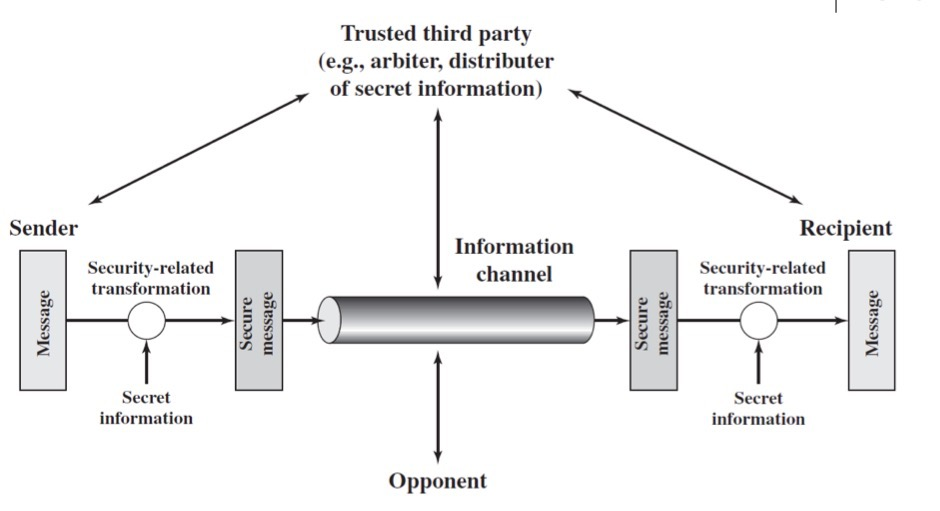
\includegraphics[width = 0.5\textwidth]{images/ModeloSeguridad}
\end{center}

La NIST define la seguridad como la triada CIA: Confidentiality, Integrity y Availability:

	\begin{itemize}
		\item Confidencialidad: Protección del acceso (o revelación) a la información solo para personas autorizadas, incluyebndo medios para proteger privacidad e información de propietario. Una pérdida de confidencialidad supone la revelación no autorizada de información
		\item Integridad: PRotección frente a modificación o destrucción de inforamción de forma no autorizada (incluye no repudio y autenticidad). Una pérdida de integridad supone la modificación o destrucción no autorizada de información.
		\item Disponibilidad: Asegurar el acceso y la utilización a tiempo y de forma confiable a la información. Una pérdida de disponibilidad supone la interrupción en el acceso o utilización de una información o sistema de información.
		\item Autenticidad: Propiedad de ser genuino y con capacidad para ser verificado y confiable. Confiabilidad en la validez de una transmisión. Que se pueda verificar que los usuarios son quienes dicen ser, o que las entradas a un sistema proceden de una fuente confiable.
		\item Contabilidad: Como no es posible que los sistemas sean completamente seguros, las partes autorizadas deberían disponer de mecanismos para trazar eventos de seguridad. Los sistemas deben almacenar registros de sus actividades para permitir análisis forenses posteriores para ayudar en la resolución de conflictos.
		\item Proporciona no repudio, disuasión, detección y prevención de intrusión, y posibilita reuperación y acciones legales posteriores.
	\end{itemize}
	
\textbf{Activos, amenazas y ataques}

\begin{center}
	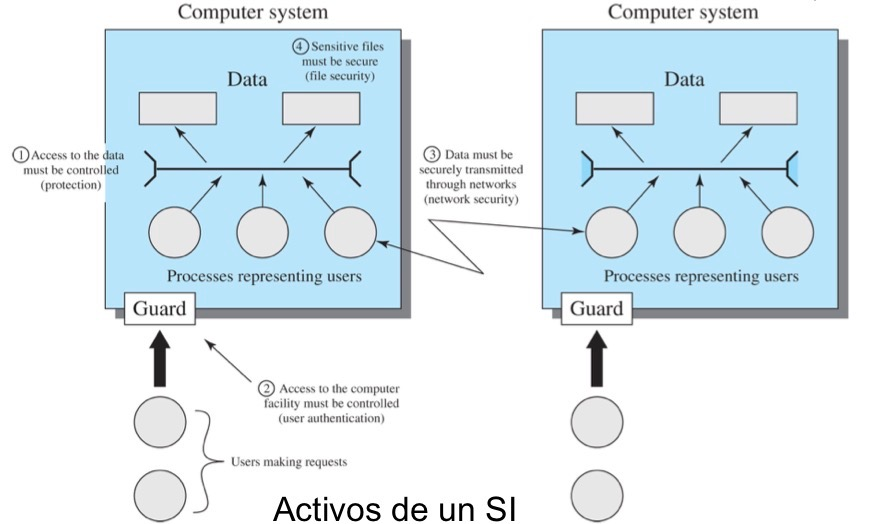
\includegraphics[width = 0.5\textwidth]{images/Activos}
\end{center}	

	\begin{itemize}
		\item \textbf{Amenazas}: "\textit{Condición del entorno de sistema de información que, dada una oportunidad, podría dar lugar a que se produjese una violación de la seguridad}".
		\item \textbf{Ataque}: "\textit{Un ataque es la realización de una amenaza}".
	\end{itemize}
	
Una \textbf{amenaza a la seguridad} es la posibilidad de violación de seguridad, que existe cuando una entidad, circunstancia que puede causar daños. Un peligro que se deriva de una posible explotación de una vulnerabilidad. Para estudiar los tipos de amenazas se suele partir de la consideración que la función de un SI es proporcionar información, se considera que hay un flujo de información de una fuente a un destino.

\begin{center}
	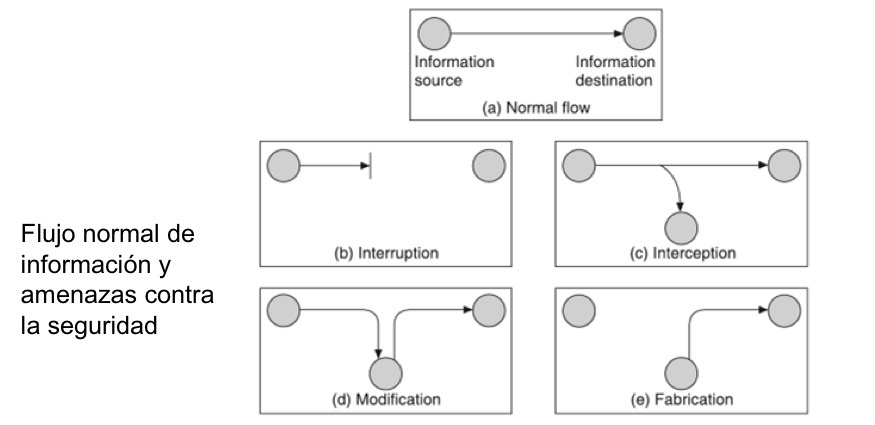
\includegraphics[width = 0.5\textwidth]{images/Amenaza}
\end{center}


\subsection{Técnicas Criptográficas}

	\subsubsection{Introducción a la criptografía}
	
	\begin{itemize}
		\item \textbf{Esteganografía} tiene como objetivo ocultar el mensaje.
		\item \textbf{Criptografía}: Objetivo es ocultar el significado del mensaje, el proceso se conoce como codificación.
		\item \textbf{Criptología}:; Ciencia que trata los problemas teóricos relacionados con la seguridad en el intercambio de mensajes en clave entre un emisor y un receptor a través de un canal de comunicaciones. Criptografía + Criptoanálisis.
		\item \textbf{Criptografía}: Técnicas de cifrado o codificado destinadas a alterar las representaciones lingüísticas de mensajes con el fin de hacerlos ininteligibles a receptores no adecuados. Tradicionalmente asociada sólo al cifrado.
	\end{itemize}
	
	\textbf{Elementos clave del sistema}: Texto en claro y texto cifrado, algoritmo de cifrado/descifrado y clave de cifrado ($K_A$) y descifrado ($K_B$).
	
	Los sistemas criptográficos se caracterizan en función de:
	
	\begin{itemize}
		\item Tipo de operaciones utilizadas para transformar el plaintext en ciphertext: sustitución y transposición.
		\item Número de claves utilizadas: simétrica y asimétrica.
		\item Forma en la que se procesa el plaintext: Bloque y stream.
	\end{itemize}
	
	Tipos básicos de cifrado en función del tipo de operaciones:
	
	\begin{itemize}
		\item Sustitución: Las unidades de texto plano son sustituidas con texto cifrado siguiendo un sistema regular. Las unidades pueden ser una sóla letra o grupos más grandes. El receptor descifra el texto realizando la operación inversa. Hay varios tipos:
			\begin{itemize}
				\item Simple: Opera sobre letras simples. Hay mono alfabético, si la sustitución es simple para todo el mensaje, y polialfabético, si utiliza diferentes sustituciones en diferentes partes de un mensaje.
				\item Poligráfico: Opera sobre grupos de letras.
			\end{itemize}
		\item Transposición: Las unidades del texto plano son cambiadas usando una ordenación diferente y normalmente bastante compleja, pero las unidades en sí mismas no son modificadas. 
	\end{itemize}
	
Criptografía de clave secreta o simétrica: Se utiliza la misma clave para cifrar y descifrar.

	\begin{equation*}
		K_A = K_B = K_{AB} \hspace{10pt} K_{AB} (K_{AB}(m)))
	\end{equation*}
	
	La clave es \textbf{secreta} ($K_{AB}$) es conocida por los dos participantes de la comunicación.\\
	
Criptografía de clave pública o asimétrica: Cada usuario cuenta con un par de clave pública ($K^+$)/privada ($K^-$). Dada la clave pública, es computacionalmente inviable obtener la clave privada. La clave privada es secreta y por tanto, conocida únicamente por el propietario legítimo de la misma, mientras que la clave pública es pública, y por tanto conocida por todos.\\
\quad Todo lo que se cifra con la clave pública únicamente puede ser descifrado con la correspondiente clave privada y vice-versa.

	\begin{equation*}
		K^+(K^-(m))) = m \hspace{10pt} \text{ó} \hspace{10pt} K^-(K^+(m))) = m
	\end{equation*}
	
Para garantizar la confidencialidad de los mensajes enviados, todos los emisores han de cifrar los mensajes con clave pública del usuario de destino y sólo será el usuario de destino que podrá descifrar el mensaje.
	
\textbf{Criptoanálisis} es la parte de la criptología que se dedica al estudio de sistemas criptográficos con el fin de encontrar debilidades en los sistemas y romper su seguridad. Buscar romper o forzar el código. Hay varios tipos de ataques según el conocimiento previo del atacante:

	\begin{itemize}
		\item \textbf{Ataques \textit{ciphertext-only}}: Cuando sólo se dispone del texto cifrado. Por ejemplo: Fuerza bruta, análisis de frecuencias o método Kasiski.
		\item \textbf{Ataque \textit{known-plaintext}}: El atacante conoce el texto original. En ocasiones, el atacante conoce una parte del texto o alguna palabra probable.
		\item \textbf{Ataque \textit{chosen-plaintext}}: El atacante tiene la capacidad de definir un texto y obtener el correspondiente texto cifrado. El objetivo es poder descifrar textos que se descicfren e ese descifrador.
	\end{itemize}
	
Si un sistema es seguro frente a ataques \textit{chosen-plaintext} también es seguro frente a ataques \textit{known-plaintext} y \textit{ciphertext-only}.	
	
	\subsubsection{Cifrado}
	
El \textbf{cifrado} es la puesta en clave (\textit{ciphertext}) de un texto (\textit{plaintext}) mediante una función parametrizada por una clave. Previene ataques contra la confidencialidad.

	\begin{center}
		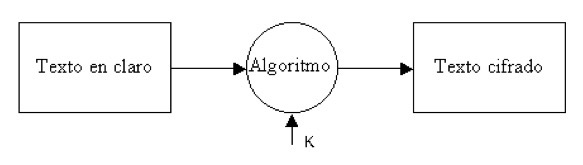
\includegraphics[width = 0.3\textwidth]{images/Cifrado}
	\end{center}

	
	
	\subsubsection{Códigos de Autenticación de Mensaje (MAC)}

	Permiten proteger la integridad y autenticidad de origen de los mensajes. Comprueban que el origen del mensaje es quién dice ser y que dicho mensaje no ha sido modificado durante su transmisión. Pueden considerarse sinónimos, si un mensaje es modificado durante su transmisión, ya no procede de su emisor légitimo sino de quien lo modificó.\\
\quad A veces puede ser necesario garantizar la integridad del mensaje pero no su confidencialida.\\

Una \textbf{función \textit{hash}} es una función que mapea cadenas de bits de longitud arbitraria a cadenas de longitud fija de $n$ bits (huella dactilar), es una función resumen y es de un único sentido. Se puede ir del texto al resumen pero en sentido inverso es imposible.\\

\textbf{MAC} (\textit{Message Authentication Code}) es un código que permite la autenticación de mensajes mediante técnicas criptográficas de clave simétrica. Los algoritmos de MAC toman como entrada dos parámetros (mensaje y clave simétrica) y generan una salida de longitud fija con la característica de que es computacionalmente inviable producir la misma salida sin conocer la clave.

	\begin{center}
		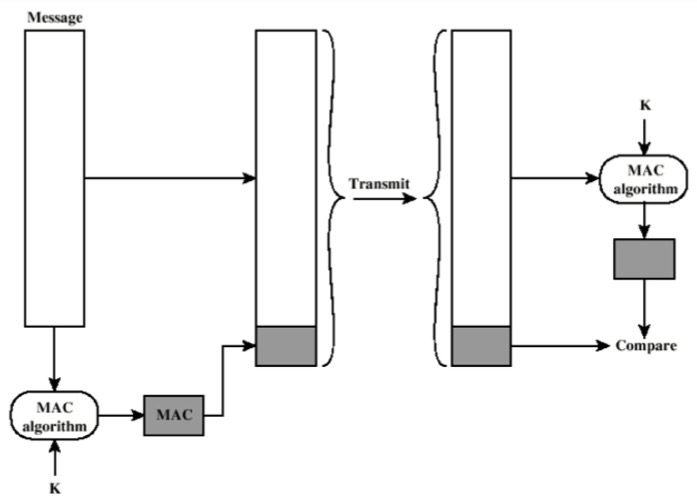
\includegraphics[width = 0.35\textwidth]{images/MAC}
	\end{center}
	
Un \textbf{ejemplo de código MAC} es HMAC (\textit{Hash-based Message Authentication Code}) y es un tipo específico de códigos MAC, el algoritmo utilizado para calcular el código MAC se basa en la utilización de funciones hash en lugar de, por ejemplo, algoritmos de cifrado.
	
		\begin{center}
		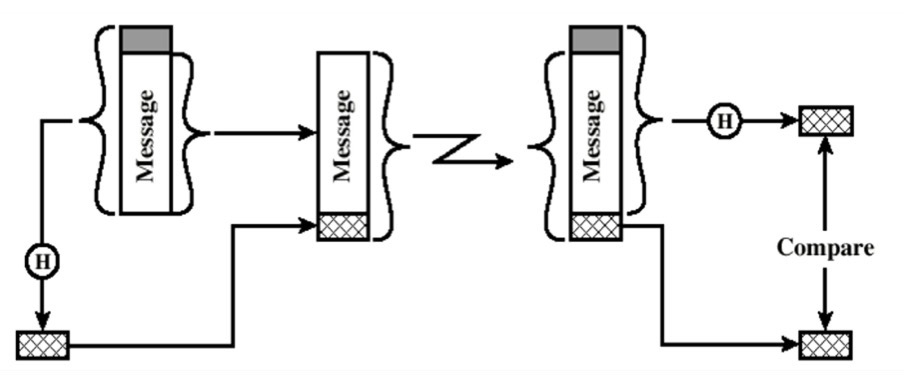
\includegraphics[width = 0.25\textwidth]{images/HMAC}
	\end{center}
	
\textbf{Características de los códigos de autenticación de mensajes}:

	\begin{itemize}
		\item Compresión: Mapean una entrada de longitud fija finita arbitraria a una salida de longitud finita fija.
		\item Facilidad de cómputo: 
	\end{itemize}
	
	\subsubsection{Firmas Digitales}
	
	
	\subsubsection{Frescura de Mensajes}
	
	
	\subsubsection{Distribución de Claves}
	

\subsection{Seguridad en SI}

\subsection{Situación Actual de la Seguridad}

\subsection{Gestión de la Seguridad}


\section{Parte 2}



\section{Parte 3}


\section{Parte 4}




































\newpage
\end{document}